\section{Evaluation}

We evaluate our counterfactual query rewriting approaches in the LongEval scenario that comes with overlapping queries accross 6~timestamps between July~2022 and August~2023~\cite{alkhalifa:2023,alkhalifa:2024,galuscakova:2023}. First, we modify the LongEval datasets to focus on queries that re-occur accross timestamps, and subsequently study how documents evolve over time due to deletions and content updates. Finally, we evaluate the retrieval effectiveness of all approaches and use an ablation study to study if they generalize beyound previously known relevant documents.

\subsection{Experimental Setup}


We noticed that queries overlap over different time slots, and in case their intent stays the same, we aim to transfer their relevance information to the new time slots. Consecutively, for those queries we know what documents were clicked a few months ago. We decided to use this feedback and query expansion with the BO1 model~\cite{amati:2003} to create keyqueries and use the same approach as \cite{froebe-mis:2022}. Thereby, we use BO1 to obtain candidate terms for query terms, as pilot experiments showed that BO1 expansion terms yield higher effectiveness than RM3~\cite{jaleel:2004} expansions. We inserted the clicked documents into the current corpus and reformulated the queries with the BO1 model until those documents were in the top positions. After that we removed old documents from the ranking. This implementation of the keyquery concept is not the most effective one, more effective approaches that leverage a generate-and-test paradigm~\cite{froebe:2021c} exist and are interesting directions for future work (i.e., explicitly generating many variants and selecting the variants that are highly effective).


\subsection{Evolution of Documents in the LongEval Corpora over Time}

Short analysis: how much did documents change? We use CopyCat~\cite{froebe:2021a}, as it was previously used to deduplicate web crawls, e.g., the ClueWebs, in default settings. ToDo: add motivation for measure and containment conceptually implemented by the S3 score.

\begin{figure}[t]
    \begin{minipage}{.49\textwidth}
        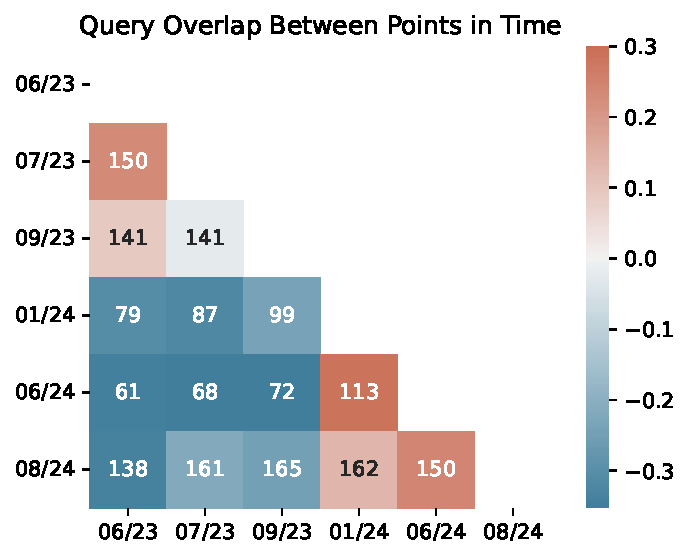
\includegraphics[width=\textwidth]{query-overlap}
        \vspace{-4ex}
        \caption{Frequency of queries and points in time.}
        \label{fig:query-overlap}
    \end{minipage}
    \hfill    
    \begin{minipage}{.49\textwidth}
        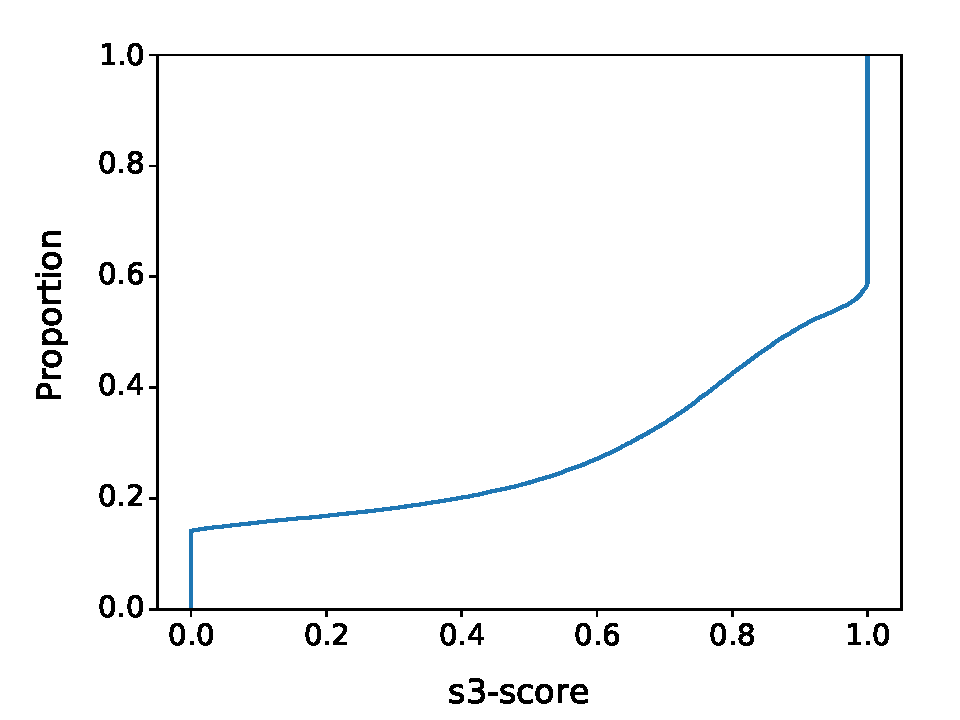
\includegraphics[width=\textwidth]{document-similarities}
        \vspace{-4ex}
        \caption{S$_{3}$ Similarities of documents with overlapping URLs as eCDF plot.}
        \label{fig:document-similarities}
    \end{minipage}
\end{figure}

% TBD.

% Approaches for comparison:

% LTR by Gijs for another approach that incorporates historical relevance data.

% Maybe few-shot prompting LLMs could be another baseline, but I would try to rather not include such baselines at the moment.


The LongEval test collections capture dynamic evaluation scenarios with different changes in all components. It evolves naturally over time, and a natural overlap between documents, queries, and qrels occurs. Since the explored approaches systematically exploit this overlap, the evaluation is challenging. Since the overlap occurs naturally in the test collection, evaluating the systems in this life-like scenario with redundancies is valid. However, we can hardly make any assumptions about how well the approaches generalize. Therefore, we include a second evaluation scenario that excludes any redundancies in the relevant documents.

  
\subsection{Baselines}
The keyqueries approach is compared to further baselines. 

We incorporate all our approaches into BM25~\cite{robertson:1994}.

For RF, we set $k=10$.


\subsection{Natural Evolving Test Collection}
In this evaluation scenario, the effectiveness is assessed in a life-like setting where the overlap naturally occurs. Thus, this setting can describe the effectiveness as it may occur in a web search scenario. Currently, the test collection covers six pints in time with, on average, 1.77 million documents. For each point in time between 407 and 1518 queries are logged and on average, 12874 qrels are constructed through the simplified Dynamic Bayesian Network (sDBN) Click Model~\cite{chapelle:2009}. The topic overlap between points in time is displayed in Figure~\ref{fig:query-overlap}, indicating that less than a third of the queries are logged repeatedly.

\begin{table}[t]
\small
\centering
\renewcommand{\tabcolsep}{3.2pt}
\caption{Retrieval effectiveness of the five baselines and our three approaches measured as nDCG@10 with and without unjudged documents (nDCG@10$^{'}$) across the five LongEval timestamps. {\color{red} $^{*}$ marks Bonferroni corrected significance for students t-test.}}
\label{tab:table-results}

\begin{tabular}{@{}l@{}cccccccccc@{}}
    \toprule
    \bfseries System & \multicolumn{5}{c}{\bfseries nDCG@10} & \multicolumn{5}{c}{\bfseries nDCG@10$^{'}$}\\
    \cmidrule(r@{.25em}){2-6}
    \cmidrule(l@{.25em}){7-11}
    
    & 07/22 & 09/22 & 01/23 & 06/23 & 08/23 & 07/22 & 09/22 & 01/23 & 06/23 & 08/23\\
    
    \midrule

    BM25 & .155 & .184 & .172 & .175 & .134 & .471 & .492 & .516 & .486 & .379 \\
    BM25$_{RM3}$ & .147 & .181 & .163 & .174 & .134 & .478 & .490 & .524 & .492 & .388 \\
    ColBERT & .198 & .207 & .201 & .184 & .151 & .402 & .409 & .420 & .408 & .315 \\
    List-in-T5 & .203 & .204 & .202 & .198 & .161 & .401 & .413 & .425 & .413 & .317 \\
    monoT5 & .202 & .219 & .197 & .202 & .154 & .405 & .410 & .415 & .411 & .314 \\
    
    \midrule
    
    BM25$_{Boost}$ & .355 & .372 & .287 & .364 & .271 & .529 & .546 & .541 & .540 & .412 \\
    BM25$_{RF}$ & .303 & .332 & .241 & .262 & .191 & .606 & .611 & .590 & .552 & .426 \\
    BM25$_{keyquery}$ & .252 & .285 & .219 & .224 & .162 & .533 & .549 & .552 & .523 & .406 \\

\bottomrule
\end{tabular}
\end{table}


\subsection{Temporal Per Topic Cross Validation}
To emphasize the actual effect of the approaches and how well they generalize to new documents, we evaluated them in a cross-validation setting. For each topic at each point in time, the relevant documents are split into $k$ folds. For each fold, only the test documents are indexed and retrieved. The different approaches can then use the documents in the train split if they were already present at the previous points in time. Since some documents can be relevant for multiple topics, the train test splits must be updated after creation to avoid duplicates. This makes the splits less random and differently large but should be neglectable for this initial evaluation.

\begin{tabular}{llrrrrr}
    \toprule
    t & Run & nDCG & nDCG@10 & bpref & P@10 & MRR \\
    \midrule
    \multirow[c]{4}{*}{$t_1$} & BM25 & 0.210 & 0.125 & 0.228 & 0.069 & 0.218 \\
    & +RM3 & 0.209 & 0.120 & 0.233 & 0.070 & 0.207 \\
    & +Bo1 & 0.217 & 0.130 & 0.238 & 0.073 & 0.219 \\
    & +RF & 0.329 & 0.251 & 0.346 & 0.114 & 0.517 \\
    & +qrel & 0.366 & 0.312 & 0.315 & 0.131 & 0.598 \\\midrule
    \multirow[c]{4}{*}{$t_2$} & BM25 & 0.258 & 0.161 & 0.269 & 0.101 & 0.254 \\
    & +RM3 & 0.256 & 0.156 & 0.266 & 0.101 & 0.246 \\
    & +Bo1 & 0.262 & 0.160 & 0.271 & 0.102 & 0.252 \\
    & +RF & 0.358 & 0.262 & 0.351 & 0.141 & 0.512 \\
    & +qrel & 0.382 & 0.309 & 0.343 & 0.158 & 0.557 \\\midrule
    \multirow[c]{4}{*}{$t_3$} & BM25 & 0.261 & 0.134 & 0.316 & 0.117 & 0.276 \\
    & +RM3 & 0.260 & 0.123 & 0.329 & 0.111 & 0.245 \\
    & +Bo1 & 0.260 & 0.130 & 0.325 & 0.118 & 0.250 \\
    & +RF & 0.346 & 0.221 & 0.393 & 0.170 & 0.543 \\
    & +qrel & 0.334 & 0.223 & 0.361 & 0.164 & 0.508 \\\midrule
    \multirow[c]{4}{*}{$t_4$} & BM25 & 0.234 & 0.139 & 0.306 & 0.116 & 0.287 \\
    & +RM3 & 0.236 & 0.141 & 0.321 & 0.123 & 0.273 \\
    & +Bo1 & 0.242 & 0.145 & 0.321 & 0.123 & 0.293 \\
    & +RF & 0.312 & 0.229 & 0.360 & 0.163 & 0.542 \\
    & +qrel & 0.343 & 0.277 & 0.354 & 0.189 & 0.606 \\\midrule
    \multirow[c]{4}{*}{$t_5$} & BM25 & 0.185 & 0.116 & 0.251 & 0.094 & 0.276 \\
    & +RM3 & 0.189 & 0.118 & 0.258 & 0.096 & 0.271 \\
    & +Bo1 & 0.187 & 0.116 & 0.256 & 0.097 & 0.261 \\
    & +RF & 0.225 & 0.162 & 0.276 & 0.119 & 0.419 \\
    & +qrel & 0.240 & 0.187 & 0.269 & 0.135 & 0.472 \\


    \bottomrule
\end{tabular}
    


